\subsection{Geometric Properties}

To gain intuition for how they might affect patterns of tag connectivity, we began by surveying geometric properties of the tag matching metrics.

\begin{figure}
\begin{center}

\begin{minipage}{0.45\linewidth}
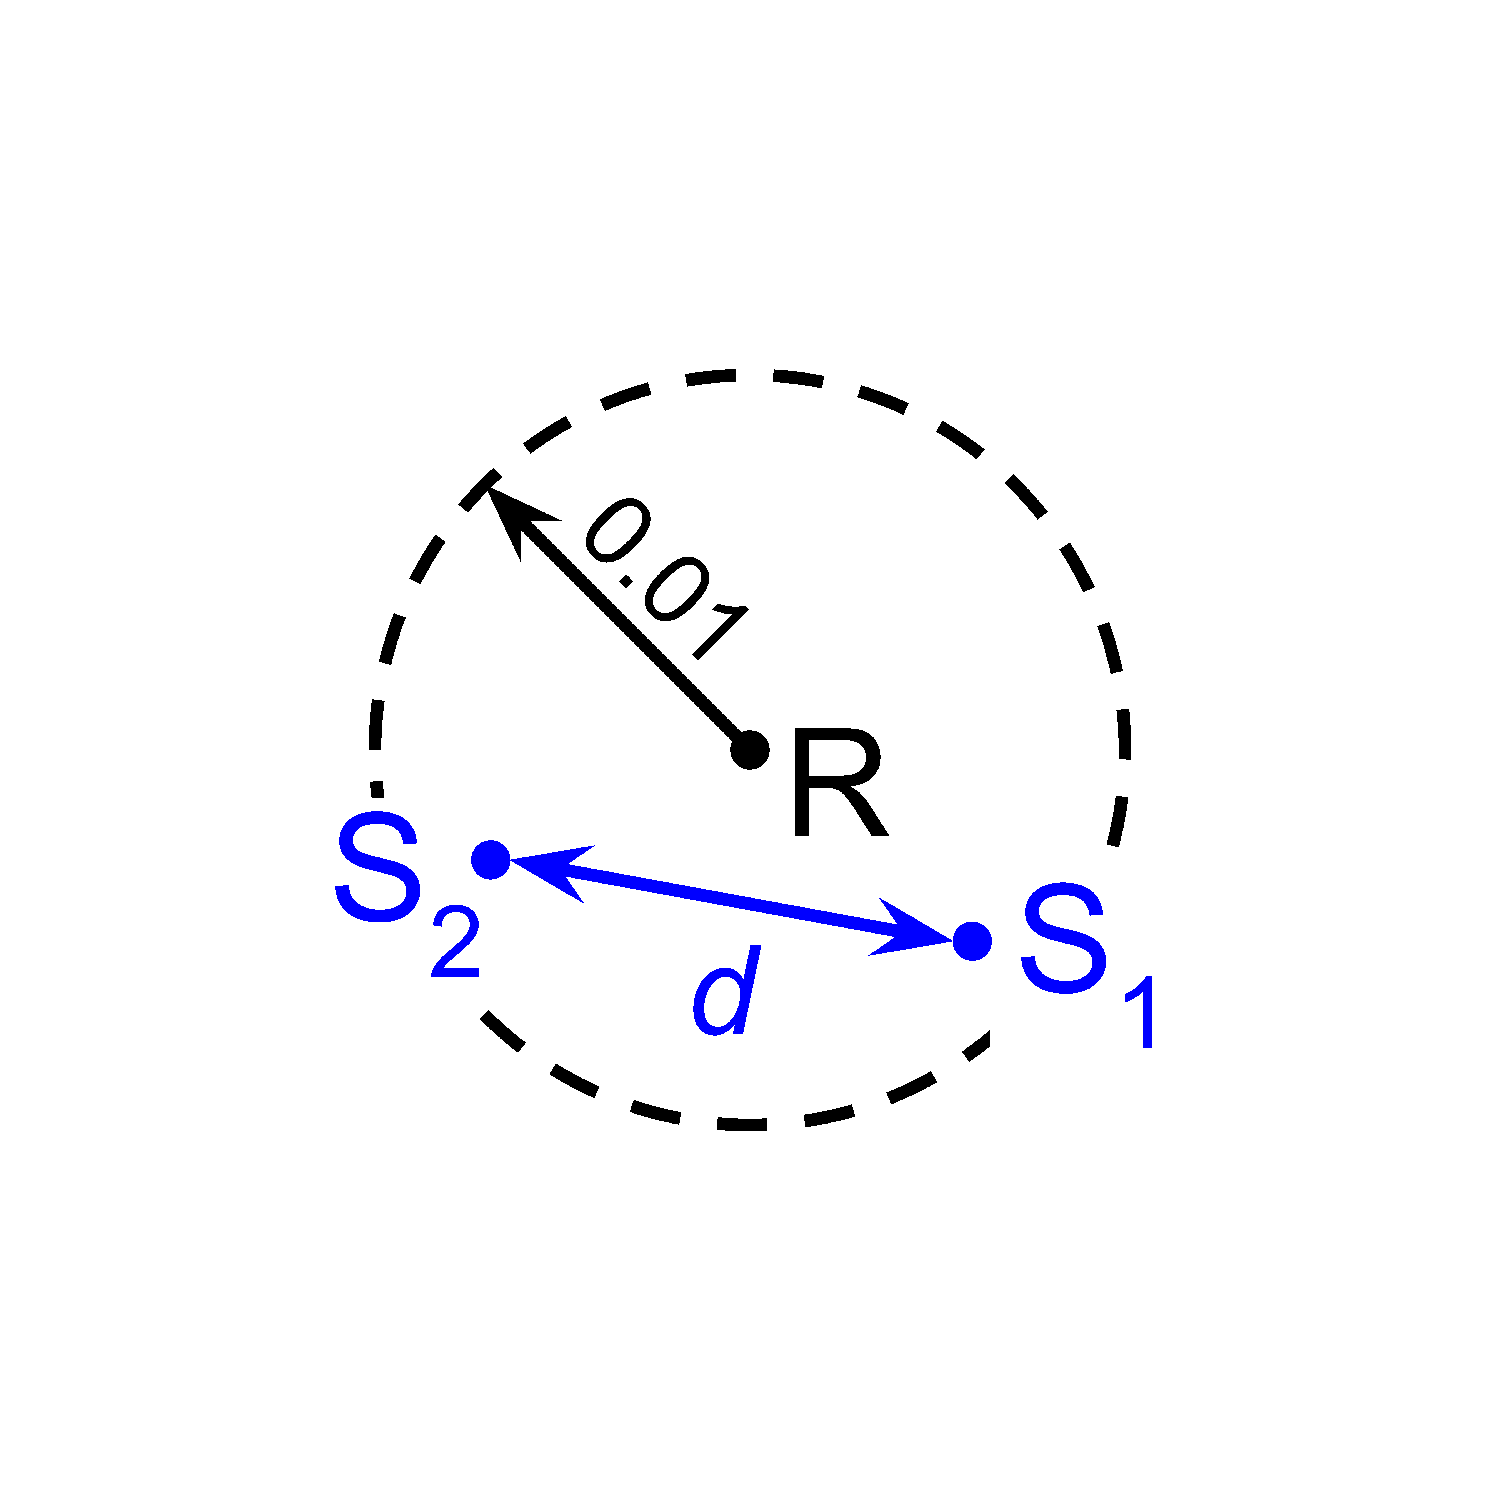
\includegraphics[width=\linewidth]{dimensionality-statistic}
\end{minipage}
\begin{minipage}{0.45\linewidth}
\caption{
The sampling process used to calculate similarity constraint for each metric.
}
\label{fig:dimensionality_measure}
\end{minipage}
\end{center}
\end{figure}


\begin{figure*}
\begin{center}

\begin{minipage}{0.15\linewidth}
\begin{subfigure}[b]{\linewidth}
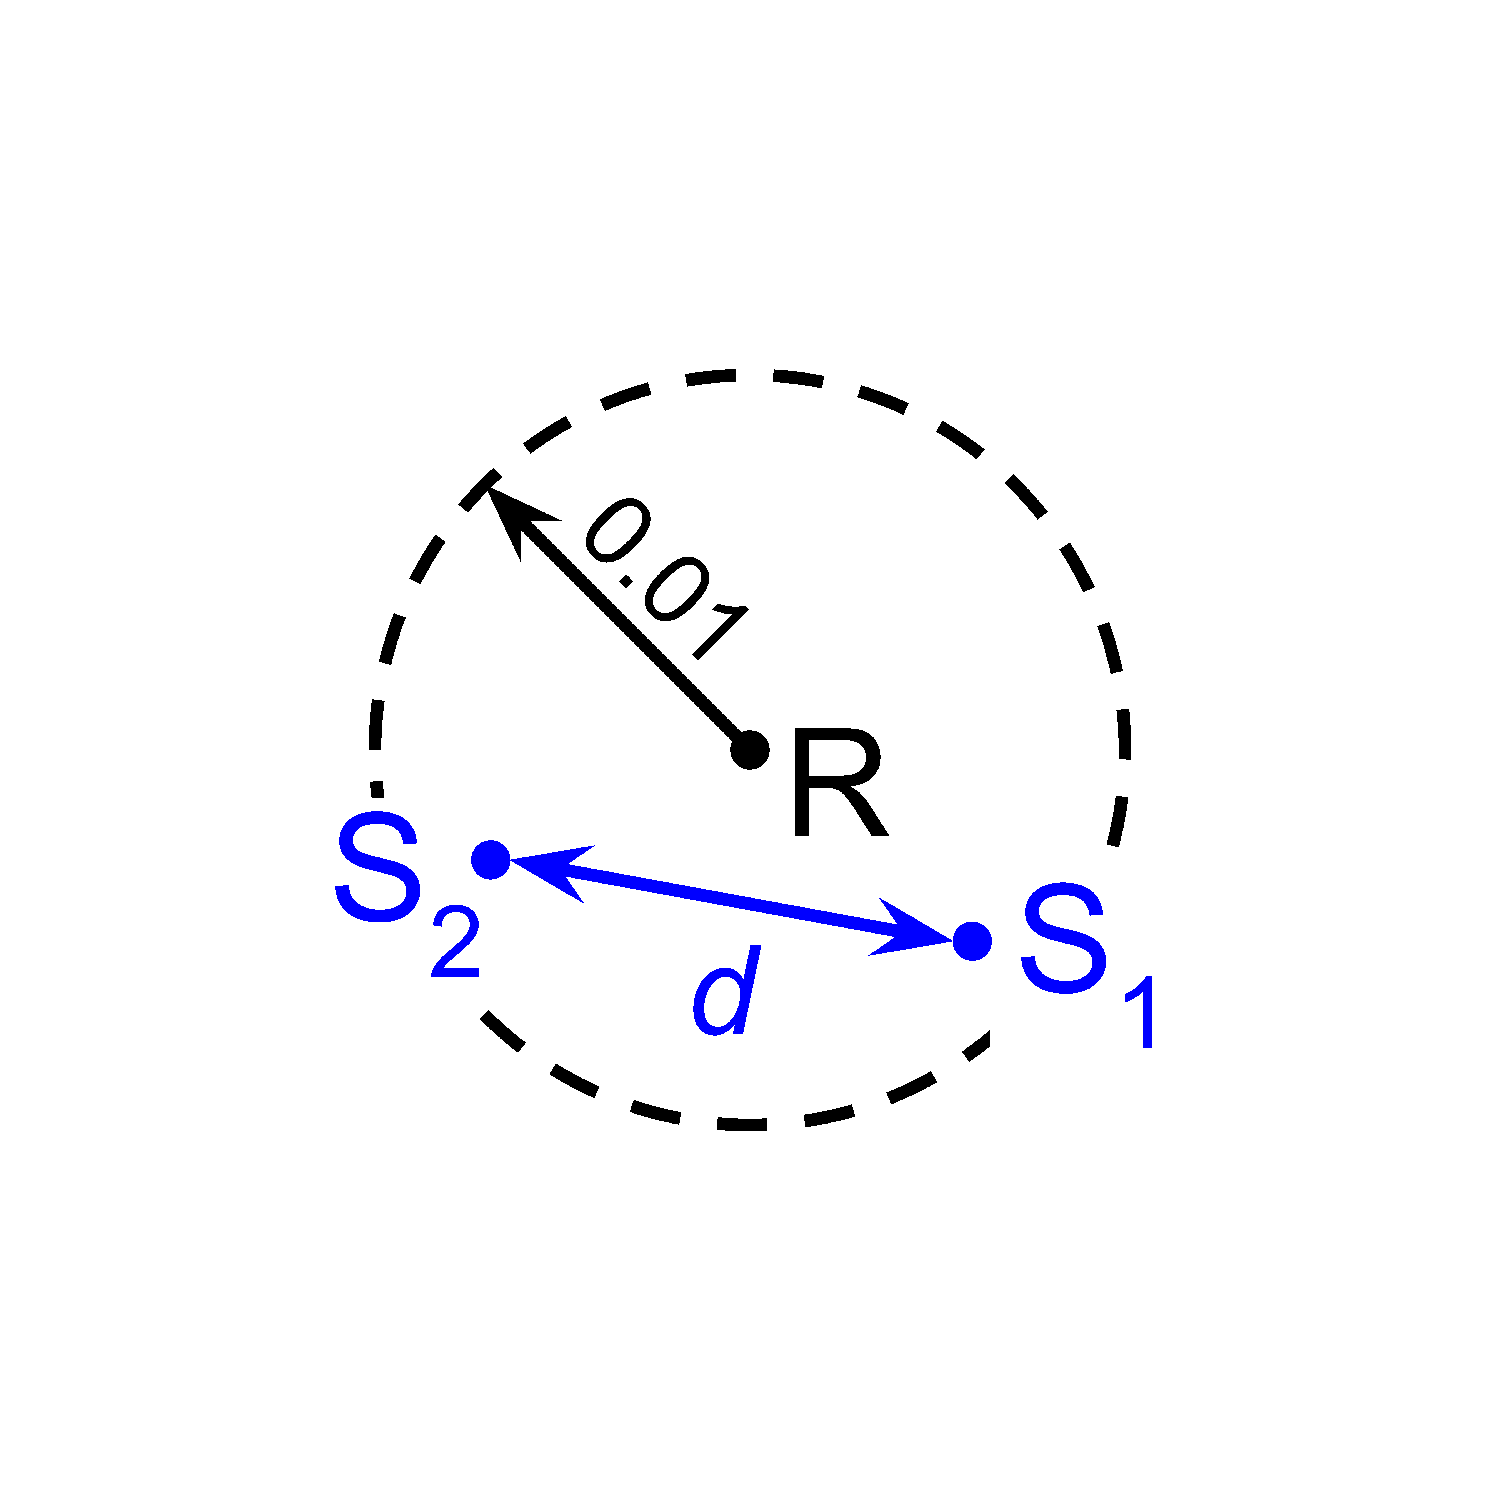
\includegraphics[width=\linewidth]{dimensionality-statistic}
\caption{
The sampling process used to calculate similarity constraint for each metric.
}
\end{subfigure}
\end{minipage}%
\begin{minipage}{0.35\textwidth}
\begin{subfigure}[b]{\linewidth}
\centering
\includegraphics[width=\linewidth]{sphere/bitweight=0dot5+seed=1+title=dimensionality_barplot+_data_hathash_hash=c0f6c5cf854ff253+_script_fullcat_hash=03ce1e318a24a109+ext=}
\caption{
Mean statistic values for each metric.
Error bars represent 95\% confidence intervals.
}
\label{fig:sphere_distnplot}
\end{subfigure}
\end{minipage}%
\begin{minipage}{0.5\linewidth}
\begin{subfigure}[b]{\linewidth}
\centering
\includegraphics[width=\linewidth]{sphere/bitweight=0dot5+seed=1+title=dimensionality_distnplot+_data_hathash_hash=c0f6c5cf854ff253+_script_fullcat_hash=03ce1e318a24a109+ext=}
\caption{
Statistic distribution, where each horizontal bar sliver represents one independent observation.
}
\label{fig:sphere_barplot}
\end{subfigure}
\end{minipage}

\caption{
Dimensionality statistic measured as distances between two tags sampled from within 0.01 match distance of a third tag.
}
\label{fig:sphere}

\end{center}
\end{figure*}


To gain a sense of the dimensionality (in a loose sense) of the different tag-matching metrics, we sampled the distribution of distances between within a 0.01 match distance radius of an arbitrary target.
We used 5000 samples.
Figure \ref{fig:dimensionality_measure}a provides a cartoon summary of this process.

In a euclidean space, this would correspond to the average distance between points uniformly sampled from inside a ball (in two dimensions, a circle, and in three dimensions, a sphere).
This statistic asymptotically increases with dimensionality (TODO show this with mathematica, also try to calculate asymptote).
In one dimension, this value approximates to 0.00666667 \citep{dunbar1997average}.
In two dimensions, 0.00905415 \citep{dunbar1997average}.
In 32 dimensions, 0.0136618 \citep{dunbar1997average}.

We calculated this statistic as  0.0067569292903519994 for the bidirectional integer metric, in line with expectations.
As you can see in Figure \ref{fig:sphere_distnplot}, the distances are all bounded by the diameter of 0.02.

However, other metrics had much higher values.
For the Spector Integer metric, we approximated this value as 0.5091638296249492.
This is an artifact of the asymmetry where if you have two very similar numbers, half will be in ascending order resulting in a match distance close to 0 and half will be in descending order, resulting in a wraparound search and a match distance close to 1.
You can very clearly see these two outcomes in \ref{fig:sphere_distnplot}.
Averaging this out yields 0.5.

The uniformified hamming had a mean distance of 0.16273783884700002.
In our sample, we observed distances as high as 0.749875.
To check our intuition, we calculated this statistic for the raw hamming metric.
For numerical reasons, we raised the radius of our sampling sphere to 0.25 (e.g., with a radius of 0.01, the only result between is a perfect match and with lower radii the hits become so rare as they become difficult to sample efficiently)
in 32 dimensional euclidean space, we expect the mean distance between sampled points to be 0.341545.
In the non-uniformified hamming metric we calculate this statistic as 0.33120625.
The distortion of the uniformification is clearly affecting this statistic with respect to the hamming metric.

We calculated an even higher value of 0.2813480713989872 for the ball sampling statistic with the streak metric.
We calculated distances as high as 0.999346.

For the hash metric, we calculated the ball sampling statistic as 0.5082513209562.
A well-behaved hash should, given any set of operands, yield hash results uniformly distributed over the range.
This case holds here.
We calculated distances as high as 0.999499.

\begin{figure}[!htbp]

\begin{center}
\begin{subfigure}[b]{\linewidth}
\begin{minipage}{0.5\linewidth}

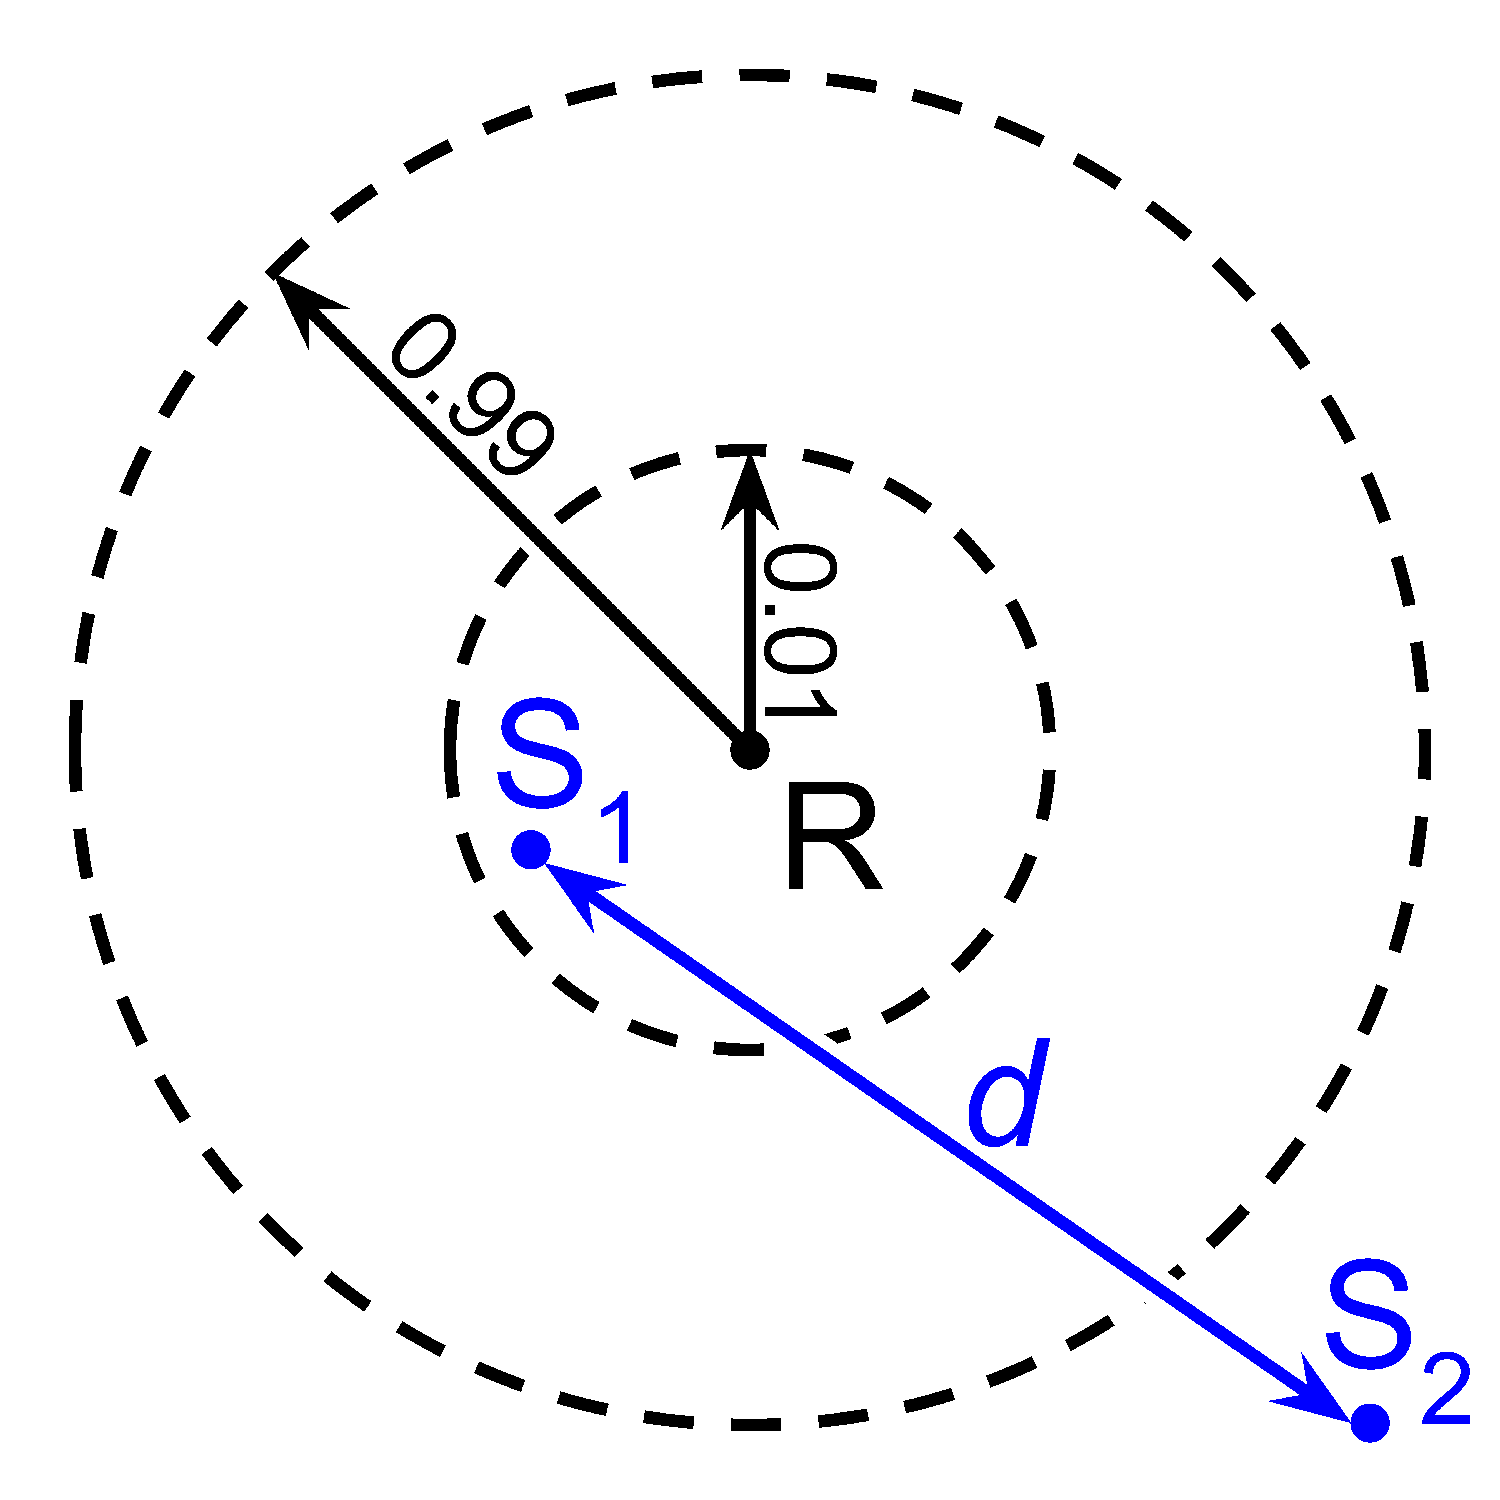
\includegraphics[width=0.75\linewidth]{img/elasticity-statistic}

\end{minipage}
\begin{minipage}{0.5\linewidth}
\caption{
Sampling process used to measure dissimilarity constraint.
First, a target tag $R$ was randomly sampled.
Then, tags were randomly drawn until a tag $S_1$ with distance to $R$ less than 0.01 was obtained.
Next, tags were randomly drawn until a tag $S_1$ with distance to $R$ more than 0.99 was obtained.
Finally, dissimilarity constraint was measured as the distance $d$ between $S_1$ and $S_2$.
}
\label{fig:dissimilarity_statistic}
\end{minipage}

\end{subfigure}

\begin{subfigure}[b]{\linewidth}
\begin{minipage}{0.6\linewidth}
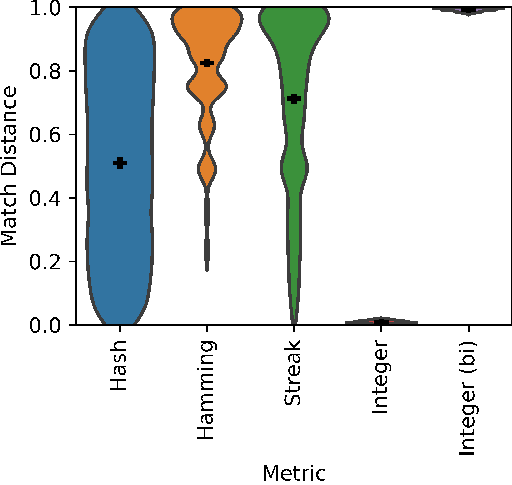
\includegraphics[width=\linewidth]{img/sphere_reverse/bitweight=0dot5+seed=1+title=dimensionality_violinplot+_data_hathash_hash=93f97a11cb443d35+_script_fullcat_hash=d1692569f79e33f8+ext=}
\end{minipage}
\begin{minipage}{0.35\linewidth}
\caption{
Mean dissimilarity constraint values for each metric.
Horizontal ticks represent means.
Error bars represent 95\% confidence intervals.
Violin plots show kernel density estimates for distribution of dissimilarity constrant.
}
\label{fig:sphere_reverse_distnplot}
\end{minipage}
\end{subfigure}
\begin{subfigure}[b]{\columnwidth}
\centering
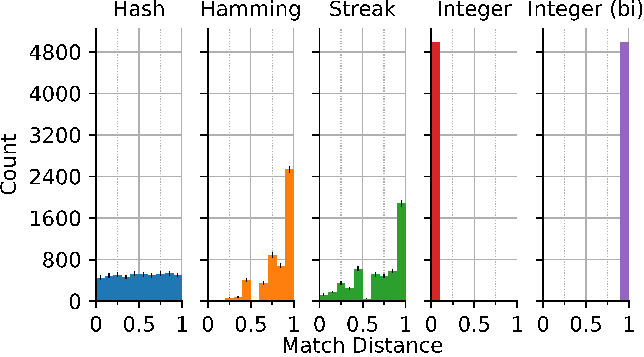
\includegraphics[width=\columnwidth]{img/sphere_reverse/bitweight=0dot5+seed=1+title=dimensionality_distnplot+viz=hist+_data_hathash_hash=93f97a11cb443d35+_script_fullcat_hash=cda229fb13f5a152+ext=}
\caption{
Frequency of sampled dissimilarity constraint values in each match distance decile.
Error bars are 95\% confidence intervals calculated using the Wilson score method with continuity correction \citep{newcombe1998two}.
}
\label{fig:sphere_reverse_barplot}
\end{subfigure}

\caption{
Dissimilarity constraint of tag-matching metrics.
Figure \ref{fig:dissimilarity_statistic} summarizes the sampling process used to measure similarity constraint.
Figures \ref{fig:sphere_reverse_barplot} and \ref{fig:sphere_reverse_distnplot} compare distributions of similarity constraint across metrics.
Supplementary Figure \ref{fig:sphere_reverse_supp} visualizes the cumulative distribution of all sampled dissimilarity constraint values for each metric.
}
\label{fig:sphere_reverse}

\end{center}
\end{figure}


We tested the elasticity of the tag-matching metrics using a similar measure.
To gain a sense of the dimensionality (in a loose sense) of the different tag-matching metrics, we sampled the distribution of distances between a tag sampled from within a 0.01 match distance radius of an arbitrary target and a tag sampled from outside a 0.99 match distance radius of the arbitrary target.
We used 5000 samples.
Figure \ref{fig:dimensionality_measure}b provides a cartoon summary of this process.

We found that the bidirectional integer metric was highly inelastic: the smallest distance between the sampled tags was 0.980201.
The mean distance between sampled tags was 0.9932740098.
The Spector integer metric exhibited similarly uniform outcomes, except the distribution was strongly pegged to 0 because of the metric's asymmetry.
The mean statistic was 0.00998706165234.

The hamming metric exhibited greater elasticity: we observed distances between the sampled tags as low as 0.235526.
The mean distance between sampled tags was 0.8248383674.

The streak metric exhibited the greatest elasticity: we observed distances between the sampled tags as low as 0.00019998.
With this metric, a tag can have a strong attractive interaction with a second tag that a third tag it interacts attractively strongly with has a strong repulsive attraction with.
The mean distance between sampled tags was 0.7126656857120001.

The hash metric exhibited the same well-behaved uniform distribution as before, with a mean distance of 0.5102822773801999.

